\documentclass[journal, 10pt]{IEEEtran}
\usepackage[utf8]{inputenc}
\usepackage[spanish,es-noshorthands]{babel}
\usepackage{amsfonts}
\usepackage{amsmath}
\usepackage{graphicx}
\usepackage{url}
\def\IEEEkeywordsname{Palabras Claves}

\makeatletter
\long\def\@makecaption#1#2{\ifx\@captype\@IEEEtablestring%
\footnotesize\begin{center}{\normalfont\footnotesize #1}\\
{\normalfont\footnotesize\scshape #2}\end{center}%
\@IEEEtablecaptionsepspace
\else
\@IEEEfigurecaptionsepspace
\setbox\@tempboxa\hbox{\normalfont\footnotesize {#1.}~~ #2}%
\ifdim \wd\@tempboxa >\hsize%
\setbox\@tempboxa\hbox{\normalfont\footnotesize {#1.}~~ }%
\parbox[t]{\hsize}{\normalfont\footnotesize \noindent\unhbox\@tempboxa#2}%
\else
\hbox to\hsize{\normalfont\footnotesize\hfil\box\@tempboxa\hfil}\fi\fi}
\makeatother

\newtheorem{example}{Ejemplo}

\begin{document}
\title{\textit{Knight's Tour:  El problema del Caballo}}
\author{Ignacio Figueroa Ram\'irez \\Sebasti\'an Herrera Corrales\\ Felipe Samur Sansur\\ Universidad T\'ecnica Federico Santa Mar\'ia \\ Avenida Vicu\~na Mackenna 3939,San Joaqu\'in, Santiago, Chile \\
\{ignacio.figueroara, sebastian.herrerac, jorge.samur\}@sansano.usm.cl\\
Longitud máxima: 2 planas}
\maketitle

\begin{abstract}
\textbf{El protagonista de este artículo es el \textit{Knight's Tour Problem}, un antiguo problema matemático que ha día de hoy sigue siendo de interés, debido a que gira en torno al caballo del ajedrez (la pieza que sin duda tiene el movimiento más curioso del set), y a la interminable cantidad de soluciones distintas que se le han encontrado. En el artículo se verá un pequeño repaso histórico del problema y conceptos relacionados, y se verá en profundiad en qué consiste el problema y como puede ser abordado y solucionado de distintas maneras gracias al aporte de distintos emblemáticos personajes de la matemática. }
\end{abstract}

\begin{IEEEkeywords}
Knight's Tour Problem, Leonhard Euler, Camino Hamiltonian, Regla de Warnsdorff.
\end{IEEEkeywords}

\section{Introducci\'on}
El \textit{Knight's Tour Problem} (KTP), o Problema del Caballo, tiene como objetivo encontrar una ruta o camino en un tablero de ajedr\'ez tal que el caballo visite todas las celdas del tablero una sola vez.
El primer \textit{problema del caballo} data del siglo septimo en un manuscrito \'arabe titulado \textit{La delicia de los inteligentes, una descripci\'on del ajedrez} y contiene dos soluciones \cite{Murray:1913}. Sin embargo, no fue hasta 1766 que el problema fue analizado por primera vez en un articulo matem\'atico \cite{Euler:1759} por el conocido Leonhard Euler, art\'iculo que sento bases para ensayos futuros. El concepto de este problema puede ser aplicado en procesamiento de imagenes, dado que el tablero de ajedrez puede emular una matriz de pixeles \cite{Xiaoyong:2017}.\\
En las siguientes secciones se profundizara m\'as acerca de este problema. En la secci\'on $II$ se profundizar\'a acerca de los movimientos que puede realizar el caballo, se presentar\'a el problema y se explicar\'a mas detalladamente con un ejemplo. La secci\'on $III$ se concentrara en [falta]. Finalmente se presentar\'an conclusiones y expectativas para el desarrollo de este problema es futuros informes.
%Fundamentación histórica del problema. No olvide citar sus fuentes . Desarrolle en prosa respondiendo las siguientes preguntas: ¿Sobre qué necesidad fue construido el problema? ¿Cuál es su origen? ¿Qué busca solucionar? ¿Por qué se hace interesante resolver el problema? ¿Cómo se aplica en la vida real? Además, no olvide mencionar que abarcará en ésta entrega y cómo estará estructurado el artículo a partir de la siguiente sección (20 pts.).

\section{El Problema}
De los seis trebejos del juego de ajedrez, en el presente articulo nos concentraremos en uno y en un problema preciso asociado a este. El caballo (\textit{en ingles Knight}) tiene un movimiento inusual entre las piezas de ajedrez. Se puede desplazar dos casillas horizontalmente y una casilla verticalmente o dos casillas en posición vertical y una horizontal. Con lo cual, el movimiento completo se parece a letra "$\mathbb{L}$"  \cite{Uehara:2019}.

\begin{figure}[h]

\centering
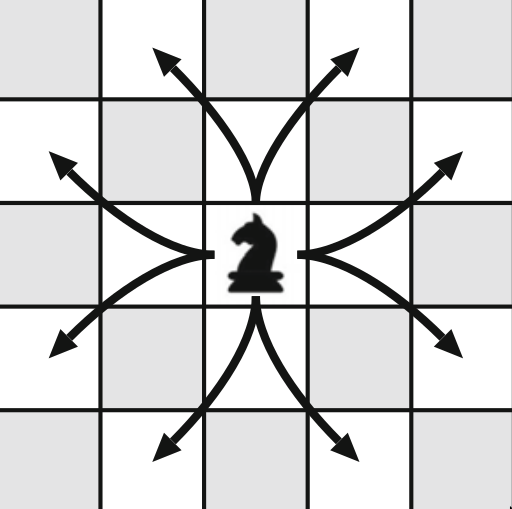
\includegraphics[width=0.2\textwidth]{figures/k_moves.png}
\caption{Movimientos del caballo en un tablero de ajedrez.}
\label{fig:moves}

\end{figure}

El problema del caballo consiste en encontrar una ruta para el caballo en un tablero de ajedrez de tamaño $8 \times 8$, de modo que este visite cada casilla una sola vez. La soluci\'on de este problema se representa como una matriz numerada que indica el orden que siguio el caballo para completa el camino, se conoce como \textit{Knight's Tour Matrix} \cite{Kopec:2016}.

\begin{figure}[h]

\centering
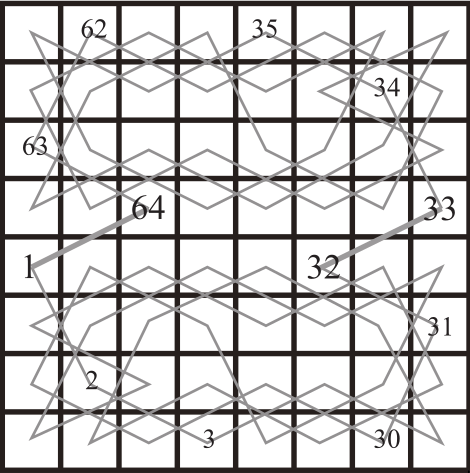
\includegraphics[width=0.2\textwidth]{figures/EulerKT.png}
\caption{Soluci\'on propuesta por Euler en 1759.}
\label{fig:euler}

\end{figure}

\begin{example}
	Una de las soluciones que encontro Euler y que publico en \cite{Euler:1759} es especialmente interesante ya que trabaja con las simetrias del tablero. Euler primero realiza un recorrido  por la mitad inferior del tablero, comenzando en el cuadrado 1 y terminando en el cuadrado 32. Luego repite exactamente este mismo recorrido, de manera sim\'etrica, para la parte superior mitad del tablero, comenzando en el cuadrado 33 y terminando en el cuadrado 64. El ejemplo se puede ver claramente en la \textit{Figura\ref{fig:euler}} 
\end{example}


%En que consiste el problema, sobre que necesidad fue construido y comentarios generales. Preguntas claves: ?`En que consiste mi problema??`Cuales son sus origines??`Que quiero solucionar? (10 ptos) .\\

\section{Estado del arte}
Con el trabajo de ordenadores se ha descubierto que el problema puede ser solucionado de más de 33 billones de maneras distintas. Distintos matemáticos han aportado su grano de arena al presentar su idea para resolverlo, como por ejemplo el anteriormente mencionado Euler. Hay soluciones que tienen todo tipo de enfoques; pueden ser para tableros de una dimensión fija, otras soluciones pueden servir para cualquier dimensión otorgada al tablero, otros solo para casos pequeños, otros dentro de un rango de dimensiones, etc. A continuación se muestran algunos algoritmos que se han diseñados para resolver el problema a lo largo de la existencia del enigma matemático:\\
\\\textbf{Warnsdorff’s algorithm for Knight’s Tour}\\
El Algoritmo de Warnsdorff funciona para tableros con dimensión minima de $5x5$, y consiste en visitar las casillas menos asequibles lo más pronto posible con la finalidad de evitar posibles caminos sin salida y/o arrinconados en un futuro. La Regla de Warnsdorff\cite{Squirrel:1996}, dice que:\\
\\Habiendo iniciado el camino de una casilla arbitraria: sea la (n+1)-ésima casilla del camino (siendo n la cantidad actual de casillas recorridas), entonces esta casilla:\\
\\1. Está al alcance de la n-ésima casilla.\\
2. Aún no ha sido visitada previamente.\\
3. Es la casilla desde la cual menos movimientos es posible hacer de todas las casillas alcanzables no visitadas de la n-ésima casilla.\\
\begin{figure}[h]
\centering
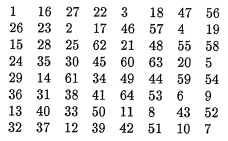
\includegraphics[width=0.2\textwidth]{figures/warnsdorff.png}
\caption{Soluci\'on hecha siguiendo la Regla de Warnsdorff}
\label{fig:euler}
\end{figure}
\\Sin embargo, pueden existir varias ocaciones en que 2 casillas cumplan con las mismas condiciones. Aquí es donde nace la imperfección del algoritmo, pues si bien existen criterios de desempate que han sido creados después de numerosos estudios del algoritmo y tienden a permitir elegir el camino correcto, no son metodologías del todo exactas y pueden aún asi originarse dilemas difíciles de resolver a la hora de elegir un camino, y si se toma una mala decisión el camino podría no terminarse. Además, la regla de Warnsdoff no es confiable por si sola para tableros de muy grandes dimensiones (p.e. $n \geq 200)$, pues estos enfrentamientos de desempate se hacen más recurrentes. Aún así, la Regla de Warnsdorff es bastante efectiva para los rangos sugeridos y una buena opción gracias a su patrón intuitivo y simpleza.   


 


% Desarrollo científico del problema. Investigar y recopilar información de como el problema ha sido abordado y/o solucionado. Explique las ventajas y defectos de los distintos enfoques aplicados (si es necesario se recomienda generar una tabla para resumir las técnicas y su información). \textit{Sea crítico en los defectos, y no endiose en los aciertos}. Además, comente sobre instancias (casos específicos) del problema que son reconocidos en la comunidad científica y los desafíos de solucionar éstos. No olvide mencionar sobre problemas similares, afines o análogos. Infiera como resoluciones de problemas similares pueden aportan grandes ideas para el desarrollo de su problema, pero sin ser explicito (\textit{hint: un mago no revela sus trucos de magia}). Desarrolle en prosa respondiendo las siguiente interrogantes: ¿Qué técnicas se han implementado? ¿Cuáles son sus ventajas y desventajas? ¿Qué instancias son interesantes de resolver? ¿Que otros problema han sido beneficiados de éste? ¿Que otros problemas han beneficiado a éste?. Considere que \textbf{debe} incluir referencias por cada técnica o solución analizada y mencionada (30 pts.).


\section{Conclusiones y Perspectivas}

Desarrollo de los aportes de la entrega, resultados y de los futuros pasos a seguir tanto como para las próximas entregas como para desarrollos fuera del curso. El orden es siempre, aportes y en párrafo aparte los trabajos futuros y/o perspectivas. Desarrolle en prosa respondiendo lo siguiente: ¿Cuál es el aporte del problema? ¿Qué es relevante del problema y como se puede seguir mejorando su resolución? ¿Qué se hará a futuro? ¿Qué se podría hacer a futuro? (10 pts.).

\newpage

\section{Referencias}
\bibliography{bibliografia}
\bibliographystyle{ieeetr}
\end{document}
